\documentclass[10pt]{article}
\usepackage[margin=1in]{geometry}
\usepackage{graphicx,booktabs,amsmath,xcolor}
\usepackage[hidelinks]{hyperref}
\title{Reading Robustness Before Reasoning:\\Residual-Stream Probes Predict Perturbation Robustness of Small Math LLMs}
\author{Francisco Angulo de Lafuente\\\small Independent researcher \quad \url{https://github.com/Agnuxo1}}
\date{AIMO Interpretability Challenge 2026 --- Small Models Track}
\begin{document}
\maketitle

\begin{abstract}
We ask whether a small reasoning model's robustness to meaning-preserving perturbations of a math problem is already encoded, linearly, in its internal state \emph{before} it generates. For each Small-Track model (Qwen3.5-4B, DeepSeek-R1-0528-Qwen3-8B, OLMo-3-7B-Think, Skywork-OR1-Math-7B) we run one forward pass on the prompt and fit two linear probes on the residual stream. Under leave-problem-out validation the probes reach AUROC $0.812\pm0.012$ (within-model AUROC $0.762\pm0.038$, accuracy $0.724\pm0.024$); re-selecting the configuration inside every outer split gives $0.805$ / $0.746$ / $0.720$. Text-only controls reach 0.734--0.766 AUROC and 0.565--0.731 within-model AUROC; a permutation test with 200 shuffles gives $p=0.005$. Decodability at the last prompt token is absent at layer 0, appears by 10\,\% depth and peaks at 40--45\,\%. Erasing the mid-depth probe subspace inside the forward pass does not reduce what final-layer probes read, showing that the signal is redundantly encoded rather than routed through a single linear bottleneck. The method needs no sampling and fits the 3600\,s budget with a wide margin.
\end{abstract}

\section{Task, data and protocol}
An instance is a pair (model, problem); it is \emph{robust} if the model's largest accuracy drop across perturbation families (distract, rename, rephrase, typos, domain) is $\le0.10$ and \emph{spurious} if $\ge0.25$. We pooled every public labelled source released by the organisers (\texttt{train-main-v2}, \texttt{augmented-sample-math-agg-filtered}, the baseline repository's per-family MATH measurements, \texttt{val-sample}, \texttt{aimo-interp-challenge-sample-full}). Recomputing the rule from per-family drops reproduces the official label on 156/156 rows. Problems are de-duplicated on whitespace-normalised text (an independent audit found 8 CRLF/LF twins, now merged); one row per (problem, labelling model). Result: 178 problems, 363 rows; the four Small-Track models label 95 rows over 74 problems (43 olympiad rows over 22 problems, 52 MATH rows). No evaluation data were used.

\textbf{Protocol.} Per evaluated model, 5 folds grouped by problem, 5 seeds; metrics on the model's own labels. Besides pooled AUROC we report \emph{within-model AUROC} (mean of per-model AUROCs), immune to base-rate differences between models. Controls: surface statistics (characters, \$ signs, backslashes, words), TF-IDF on 1--2-grams, input embeddings (layer-0 token mean), per-model prior, and shuffled labels. Paired bootstrap over problems (2000 resamples).

\section{Method}
\textbf{Features.} The problem is wrapped in the model's chat template with a fixed instruction (step-by-step reasoning, boxed answer) and passed once through the model (bf16, Transformers 5.13 as in the official runtime). We keep $h^{(\ell)}_{T}$, the residual stream at the last prompt token, and $\bar h^{(\ell)}=\frac1T\sum_t h^{(\ell)}_t$ for every layer.

\textbf{Probes.} Each probe is a standardiser, PCA to 16 dimensions and an $\ell_2$ logistic regression ($C=0.1$, balanced classes). The submission averages two probes: last-token states standardised per layer and averaged over the $0.4L$--$0.8L$ band, and the token mean at layer $L$. Threshold 0.5.

\textbf{Label pooling.} Own labels are scarce (9--62 per model). Each model's probe is also trained on problems labelled only by other models (one vote per labelling model, ties dropped), always on the target model's activations; validation uses own labels only.

\textbf{Selection.} Eight configurations were compared; we chose the one best on within-model AUROC and on the olympiad subset, the metrics closest to test conditions. Nested CV (selection repeated inside each outer training split with an inner 4-fold CV) quantifies the optimism of this step.

\section{Results}
\begin{table}[h]\centering\small
\begin{tabular}{lcccc}\toprule
 & AUROC & within-model AUROC & accuracy & balanced acc.\\\midrule
\textbf{Residual-stream probes (submitted)} & \textbf{0.812}$\pm$0.012 & \textbf{0.762}$\pm$0.038 & \textbf{0.724}$\pm$0.024 & \textbf{0.735}$\pm$0.024\\
\quad nested selection & 0.805$\pm$0.012 & 0.746$\pm$0.016 & 0.720$\pm$0.023 & 0.732$\pm$0.023\\
Input embeddings (layer 0) & 0.766$\pm$0.013 & 0.731$\pm$0.033 & 0.676$\pm$0.023 & 0.680$\pm$0.022\\
Surface statistics & 0.746$\pm$0.008 & 0.565$\pm$0.016 & 0.688$\pm$0.005 & 0.684$\pm$0.006\\
TF-IDF n-grams & 0.734$\pm$0.024 & 0.622$\pm$0.037 & 0.642$\pm$0.026 & 0.652$\pm$0.027\\
Shuffled labels (200 perms, max) & 0.651 & 0.723 & --- & 0.638\\\bottomrule
\end{tabular}
\caption{Leave-problem-out results, mean $\pm$ s.d. over 5 seeds. Olympiad subset: balanced accuracy $0.593\pm0.056$, AUROC $0.737\pm0.046$.}
\end{table}

\begin{figure}[t]\centering
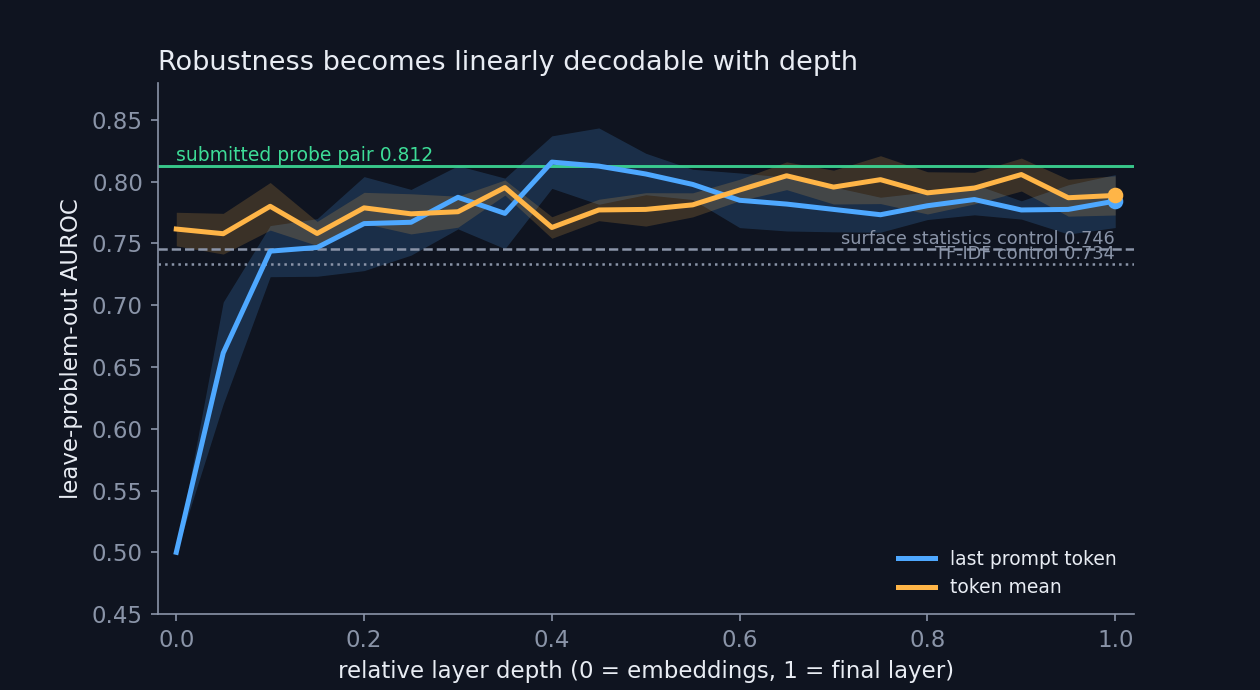
\includegraphics[width=.49\linewidth]{../figures/layer_sweep.png}\hfill
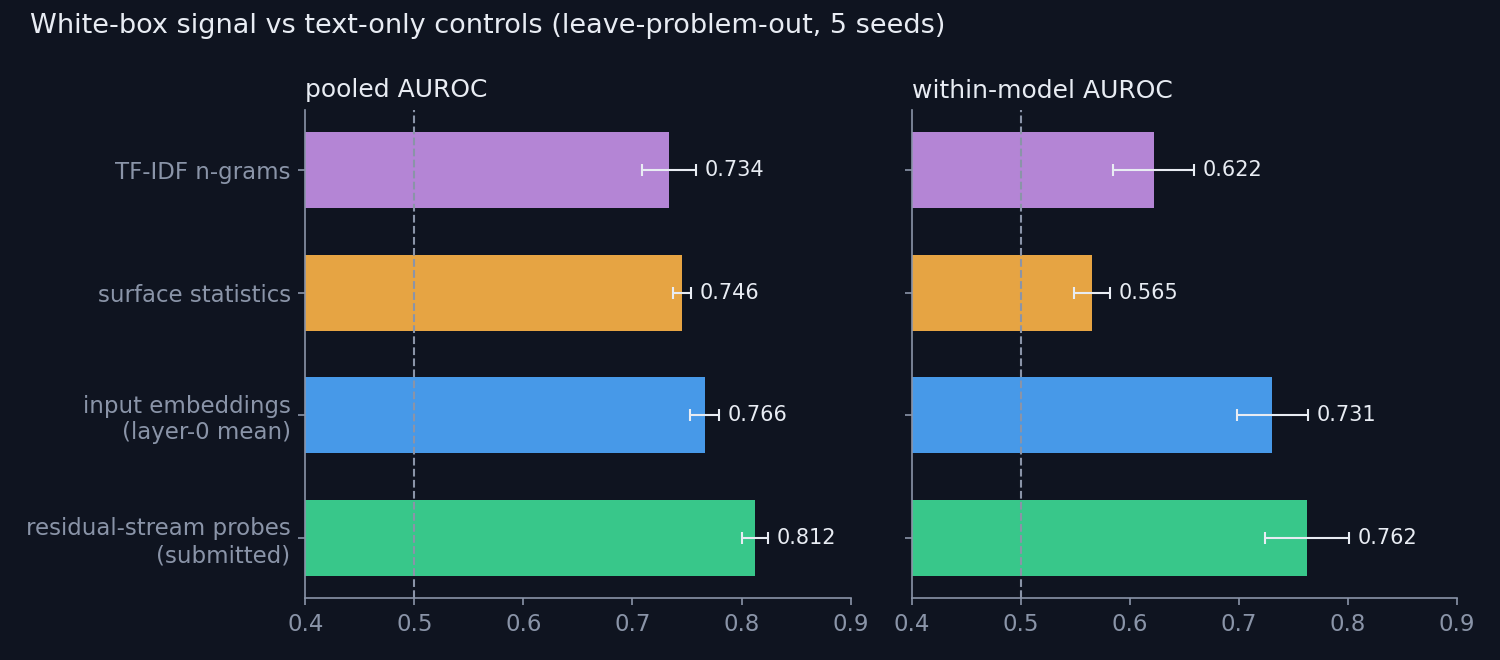
\includegraphics[width=.49\linewidth]{../figures/controls.png}\\[2mm]
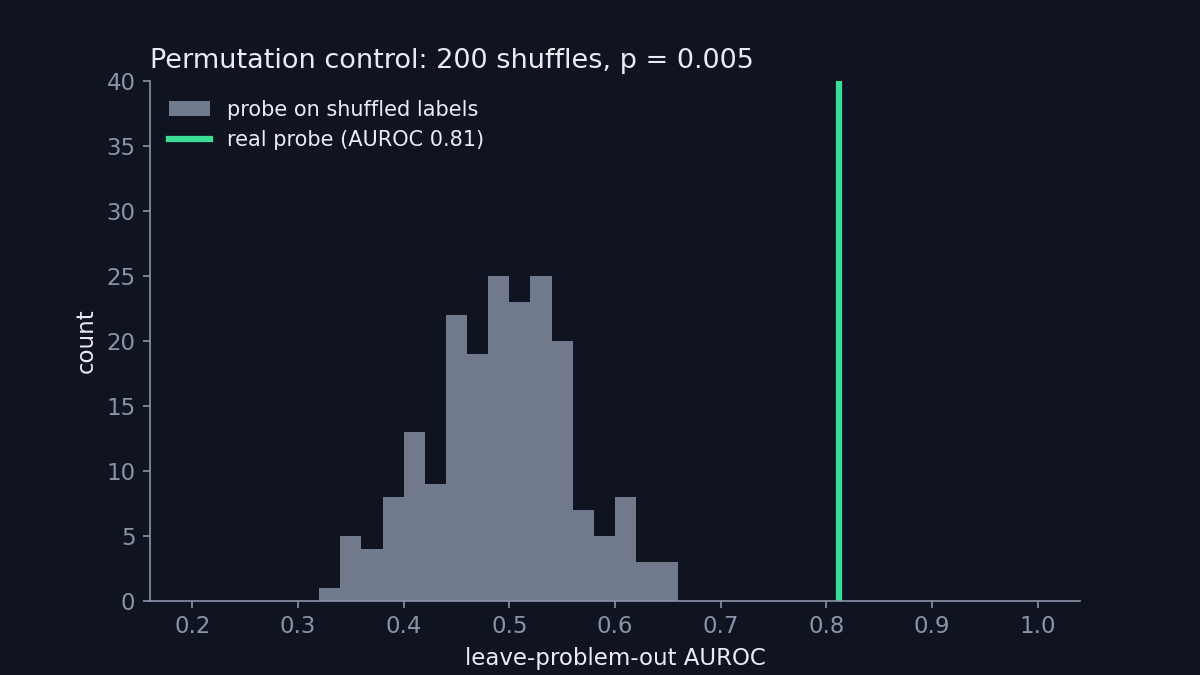
\includegraphics[width=.49\linewidth]{../figures/permutation_null.png}\hfill
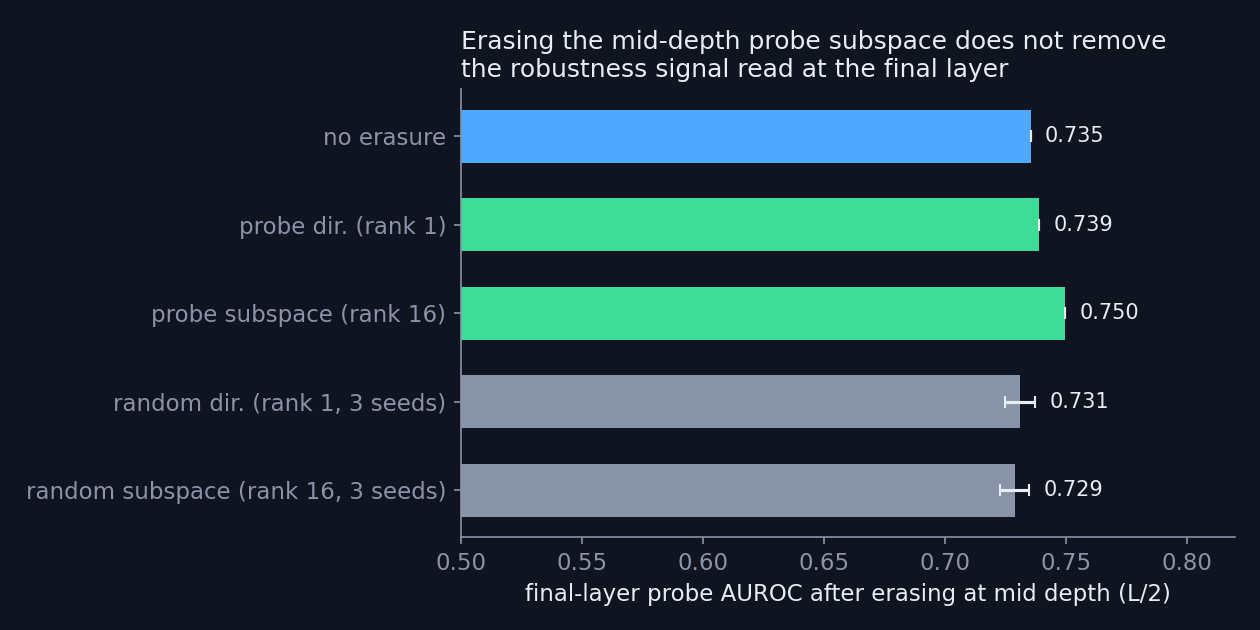
\includegraphics[width=.49\linewidth]{../figures/ablation.png}
\caption{Top left: AUROC versus relative depth. Top right: submitted probes versus text-only controls. Bottom left: permutation null. Bottom right: causal erasure at $L/2$.}
\end{figure}

\paragraph{White-box ablation.} Swapping the residual-stream features for text-only features (same classifier, same folds) lowers within-model AUROC by up to 0.20 and pooled AUROC by 0.05--0.08. Paired bootstrap at problem level (175 problems, own and problem-level labels) gives $\Delta$AUROC $=+0.052$ [$+0.002,+0.104$] against surface statistics, $+0.048$ [$-0.017,+0.111$] against TF-IDF and $+0.025$ [$-0.006,+0.058$] against input embeddings; on own labels only (74 problems) all differences are positive with wider intervals (e.g.\ $+0.128$ [$0.000,+0.249$] balanced accuracy against TF-IDF).

\paragraph{Depth.} At the last prompt token, layer 0 is identical across prompts and carries no signal by construction; AUROC reaches 0.744 at 10\,\% depth and peaks at 0.816 at 40\,\%, consistent with problem-level fragility being assembled while the prompt is processed.

\paragraph{Causal erasure.} Inside each training split we fit a token-mean probe at $L/2$, map it back to a residual direction (rank 1) or its PCA subspace (rank 16), and project it out of every token's residual stream at $L/2$ while re-running held-out problems. Final-layer probes trained on unablated activations keep their AUROC (0.735 $\to$ 0.739 / 0.750), as with random erasures of equal rank (0.723--0.736). The information is therefore redundantly encoded and re-derivable by later layers; a single linear bottleneck is rejected.

\section{Submission}
Probes are exported as NumPy arrays; \texttt{are\_robust} loads the evaluated model offline, runs one forward pass per problem and thresholds the probe average at 0.5. With the official ingestion and scoring programs on an RTX 3090, 43 cases over the four models took $\approx$165\,s including cold model loads; two runs gave identical predictions. Codabench submission IDs (Small Model Track): 1015694 (final), 1015306, 1015190.

\section*{Limitations}
Labels are scarce at olympiad level (43 rows, 22 problems), where intervals are wide. With own labels only the bootstrap intervals against controls include zero; the advantage is significant at problem level against surface statistics and modest against input embeddings, which are a strong baseline. The band standardisation uses label-free statistics of all rows in a split (measured effect $\le0.001$ on predictions). Probes are correlational; the erasure result shows redundancy, not which components use the information.

\section*{AI usage statement}
An AI coding assistant (Claude) was used to write experiment code, run analyses and draft this report under the author's direction; an independent AI verifier audited the pipeline. All numbers come from logged runs in the public repository.

\section*{Reproducibility}
Code, logs, environment and the submission bundle:\\
{\footnotesize\url{https://github.com/Agnuxo1/aimo-interp-residual-robustness-probes}}\\
Training data: the organisers' public datasets listed in Section 1; training codebase: \texttt{src/}; bundle: \texttt{submission/}.

\begin{thebibliography}{9}\small
\bibitem{aimo} AIMO Interpretability Challenge 2026. \url{https://aimo-interp.github.io/}; proposal arXiv:2607.13899.
\bibitem{alain} G.~Alain and Y.~Bengio. Understanding intermediate layers using linear classifier probes. arXiv:1610.01644, 2016.
\bibitem{belinkov} Y.~Belinkov. Probing classifiers: Promises, shortcomings, and advances. \emph{Computational Linguistics} 48(1), 2022. doi:10.1162/coli\_a\_00422.
\bibitem{hewitt} J.~Hewitt and P.~Liang. Designing and interpreting probes with control tasks. EMNLP 2019. doi:10.18653/v1/D19-1275.
\bibitem{leace} N.~Belrose et al. LEACE: Perfect linear concept erasure in closed form. NeurIPS 2023. arXiv:2306.03819.
\bibitem{gsm} I.~Mirzadeh et al. GSM-Symbolic: Understanding the limitations of mathematical reasoning in LLMs. arXiv:2410.05229, 2024.
\bibitem{kadavath} S.~Kadavath et al. Language models (mostly) know what they know. arXiv:2207.05221, 2022.
\bibitem{marks} S.~Marks and M.~Tegmark. The geometry of truth. arXiv:2310.06824, 2023.
\end{thebibliography}
\end{document}
